%%%%%%%%%%%%%%%%%%%%%%%%%%%%%%%%%%%%%%%%%
% Beamer Presentation
% LaTeX Template
% Version 1.0 (10/11/12)
%
% This template has been downloaded from:
% http://www.LaTeXTemplates.com
%
% License:
% CC BY-NC-SA 3.0 (http://creativecommons.org/licenses/by-nc-sa/3.0/)
%
%%%%%%%%%%%%%%%%%%%%%%%%%%%%%%%%%%%%%%%%%

%----------------------------------------------------------------------------------------
%	PACKAGES AND THEMES
%----------------------------------------------------------------------------------------

\documentclass{beamer}

\mode<presentation> {

% The Beamer class comes with a number of default slide themes
% which change the colors and layouts of slides. Below this is a list
% of all the themes, uncomment each in turn to see what they look like.

%\usetheme{default}
%\usetheme{AnnArbor}
%\usetheme{Antibes}
%\usetheme{Bergen}
%\usetheme{Berkeley}
%\usetheme{Berlin}
%\usetheme{Boadilla}
%\usetheme{CambridgeUS}
%\usetheme{Copenhagen}
%\usetheme{Darmstadt}
%\usetheme{Dresden}
%\usetheme{Frankfurt}
%\usetheme{Goettingen}
%\usetheme{Hannover}
%\usetheme{Ilmenau}
%\usetheme{JuanLesPins}
%\usetheme{Luebeck}
\usetheme{Madrid}
%\usetheme{Malmoe}
%\usetheme{Marburg}
%\usetheme{Montpellier}
%\usetheme{PaloAlto}
%\usetheme{Pittsburgh}
%\usetheme{Rochester}
%\usetheme{Singapore}
%\usetheme{Szeged}
%\usetheme{Warsaw}

% As well as themes, the Beamer class has a number of color themes
% for any slide theme. Uncomment each of these in turn to see how it
% changes the colors of your current slide theme.

%\usecolortheme{albatross}
%\usecolortheme{beaver}
%\usecolortheme{beetle}
%\usecolortheme{crane}
%\usecolortheme{dolphin}
%\usecolortheme{dove}
%\usecolortheme{fly}
%\usecolortheme{lily}
%\usecolortheme{orchid}
%\usecolortheme{rose}
%\usecolortheme{seagull}
%\usecolortheme{seahorse}
%\usecolortheme{whale}
%\usecolortheme{wolverine}

%\setbeamertemplate{footline} % To remove the footer line in all slides uncomment this line
%\setbeamertemplate{footline}[page number] % To replace the footer line in all slides with a simple slide count uncomment this line

%\setbeamertemplate{navigation symbols}{} % To remove the navigation symbols from the bottom of all slides uncomment this line
}

\usepackage{graphicx} % Allows including images
\usepackage{booktabs} % Allows the use of \toprule, \midrule and \bottomrule in tables

%----------------------------------------------------------------------------------------
%	TITLE PAGE
%----------------------------------------------------------------------------------------

\title[Revealed Preference]{Watch and Learn: Optimizing from Revealed Preferences Feedback} % The short title appears at the bottom of every slide, the full title is only on the title page

\author{Aaron Roth, Jonathan Ullman, and Zhiwei Steven Wu\footnote{This note is completed with discussion with Ruta Mehta and Matus Telgarsky.}} % Your name
\institute[] % Your institution as it will appear on the bottom of every slide, may be shorthand to save space
{
 \\ % Your institution for the title page
\medskip
\textit{} % Your email address
}
\date{\today} % Date, can be changed to a custom date

\begin{document}

\begin{frame}
\titlepage % Print the title page as the first slide
\end{frame}

\begin{frame}
\frametitle{Overview} % Table of contents slide, comment this block out to remove it
\tableofcontents % Throughout your presentation, if you choose to use \section{} and \subsection{} commands, these will automatically be printed on this slide as an overview of your presentation
\end{frame}

%----------------------------------------------------------------------------------------
%	PRESENTATION SLIDES
%----------------------------------------------------------------------------------------

%------------------------------------------------
\section{Introduction} % Sections can be created in order to organize your presentation into discrete blocks, all sections and subsections are automatically printed in the table of contents as an overview of the talk
%------------------------------------------------

\subsection{A Market model} % A subsection can be created just before a set of slides with a common theme to further break down your presentation into chunks

\begin{frame}
\frametitle{A Market Model}
One seller
\begin{itemize}
    \item has $m$ kinds of goods;
    \item has a cost function $c:\mathbb{R}_+^m\rightarrow \mathbb{R}_+$ which is \textbf{convex} and \textbf{known} to the seller;
    \item can set prices for goods.
\end{itemize}
Many buyers, the $i$-th of them
\begin{itemize}
    \item has a valuation function $v_i:\mathbb{R}_+^m\rightarrow \mathbb{R}_+$ which is \textbf{monotonically increasing}, $\boldsymbol{\alpha}$-\textbf{strongly concave}, and \textbf{unknown} to the seller;
    \item will maximize the utility $u_i(x,p)=v_i(x)-\langle x,p\rangle$ over a convex compact $\mathcal{C}\subset \mathbb{R}_+^m$ given the price vector $p$. This is called a quasi-linear utility.
\end{itemize}
\end{frame}

\begin{frame}
    \frametitle{An Explanation}
    \begin{center}
        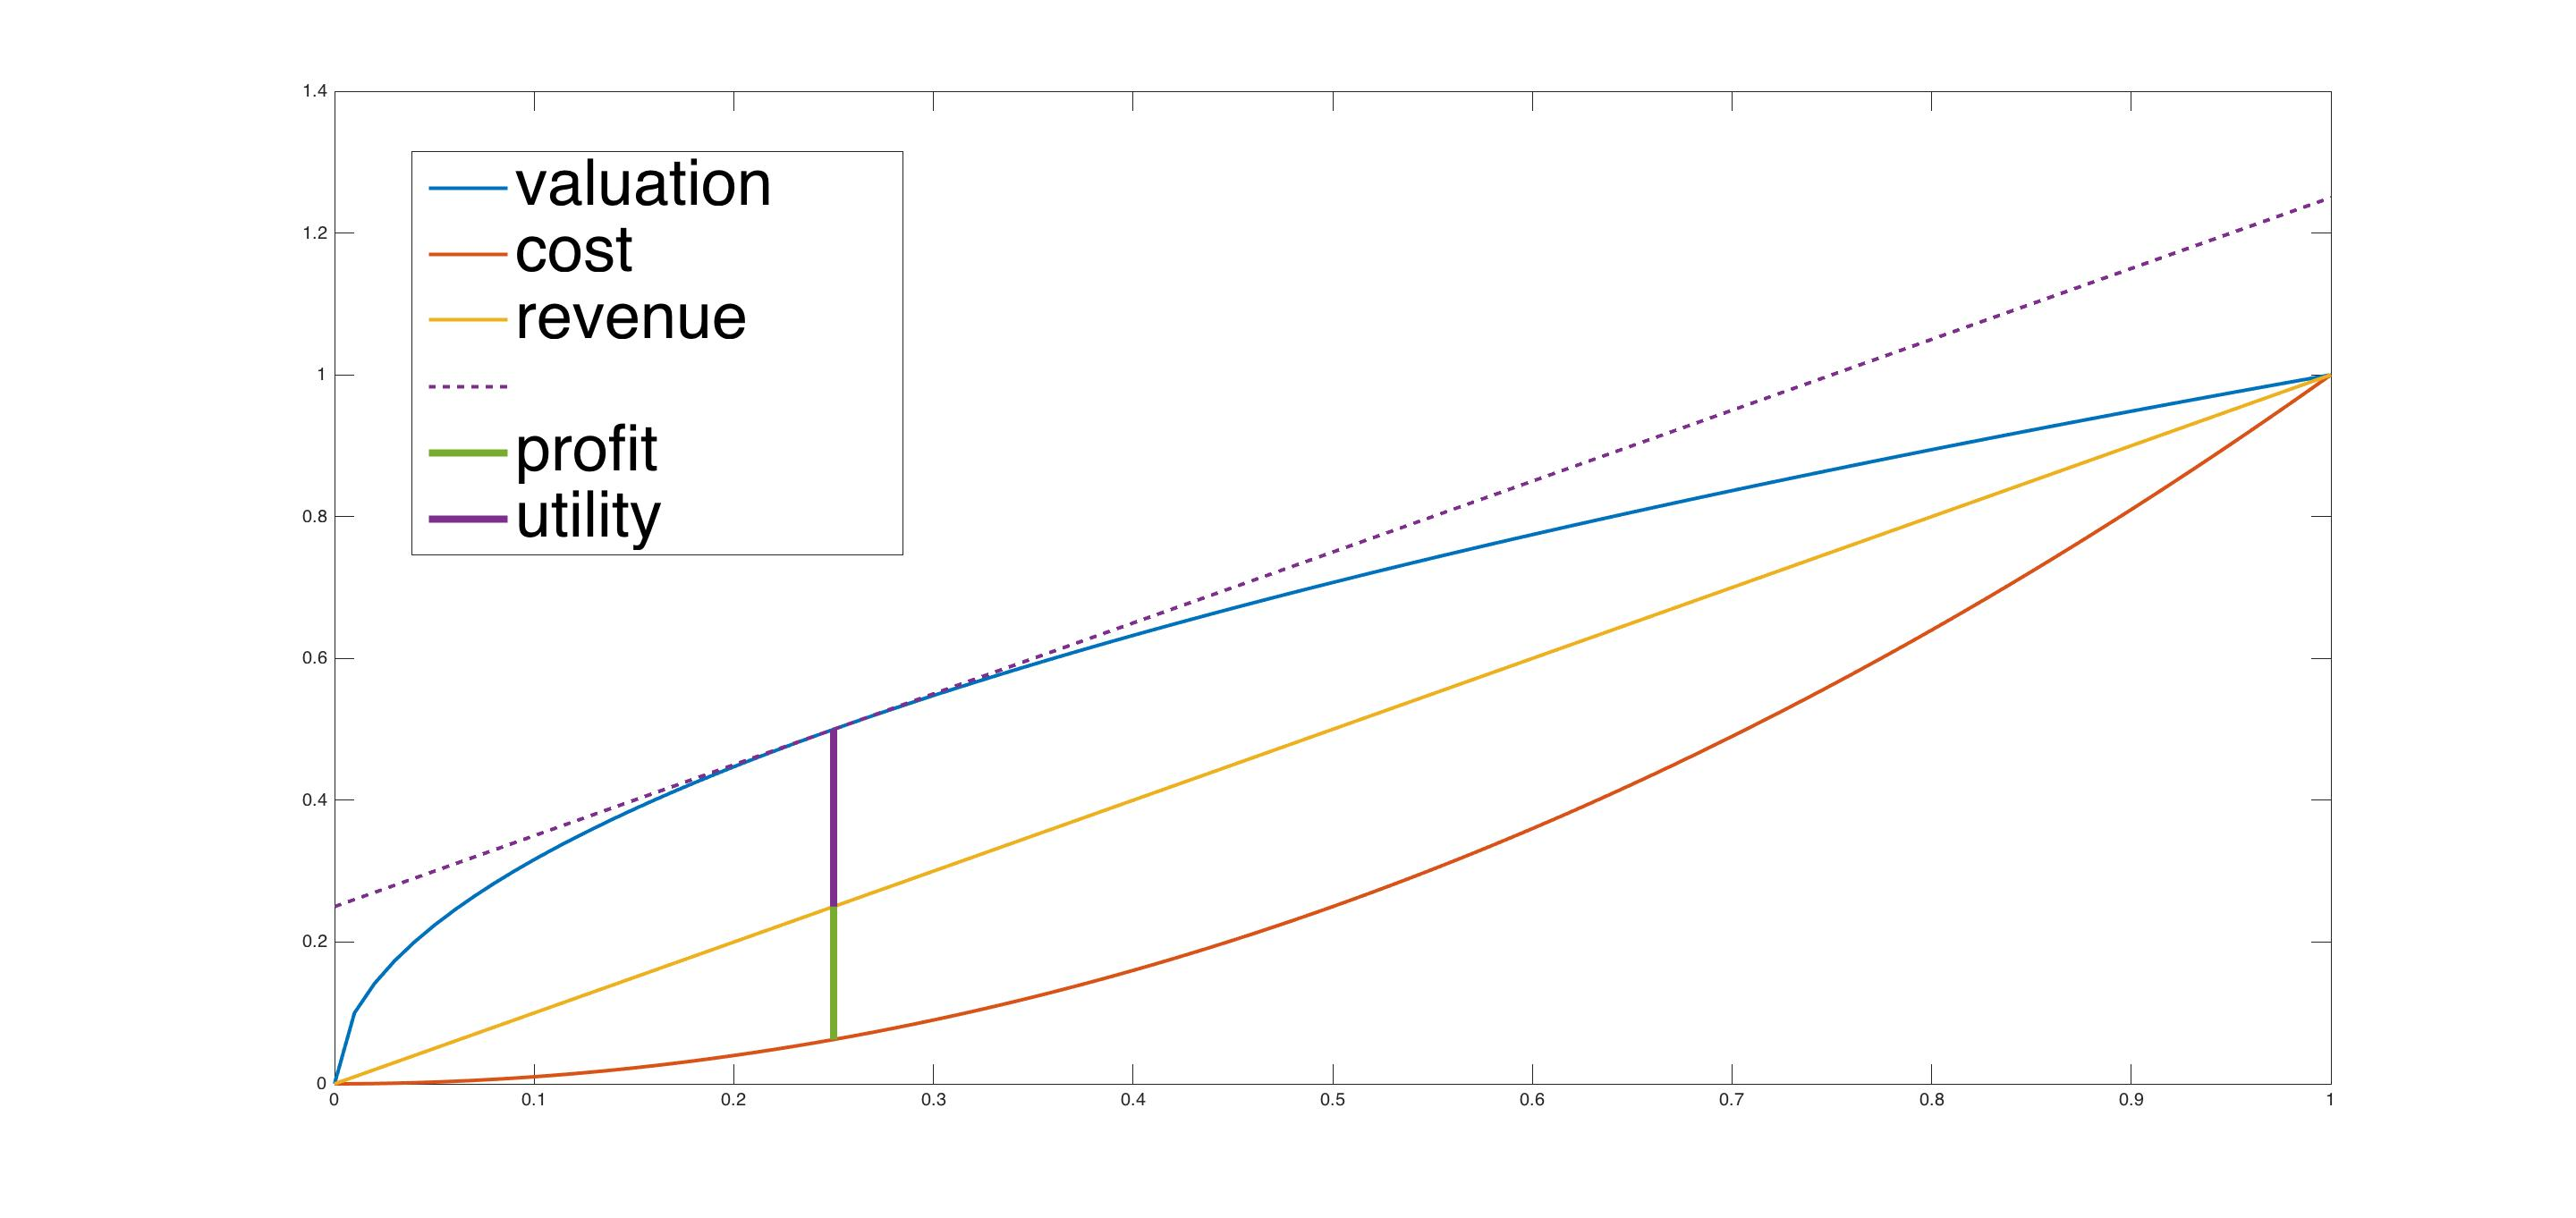
\includegraphics[width=0.8\textwidth]{market.jpg}
    \end{center}
    \begin{center}
        social welfare = buyer's utility + seller's profit
    \end{center}
\end{frame}

\begin{frame}
    \frametitle{Different Objectives}
    Set price vector $p$ in order to
    \begin{itemize}
        \item maximize profit;
        \item \textbf{maximize social welfare};
        \item learn the valuations;
        \item ...
    \end{itemize}
\end{frame}

\begin{frame}
    \frametitle{Social Welfare Maximization}
    First assume there is only one buyer.

    Given price $p\in \mathbb{R}_+^m$, let
    \begin{equation}
        x(p)=\arg\max_{x\in \mathcal{C}}u(x,p)=\arg\max_{x\in \mathcal{C}}(v(x)-\langle x,p\rangle).
    \end{equation}
    We try to maximize $\mathrm{SW}(p)=v(x(p))-c(x(p))$ over $p\in\mathbb{R}_+^m$. But we \textbf{don't know} $v$!
\end{frame}

%------------------------------------------------

\subsection{Some Convexity Results}
\begin{frame}
    \frametitle{Subgradients and Supergradients}
    For $f(x)$ and $x\in \mathbf{dom}\,f$, $p$ is called a subgradient of $f$ at $x$ if
    \begin{equation}
        \forall x'\in \mathbf{dom}\,f,f(x')-f(x)\ge p(x'-x);
    \end{equation}
    and a supergradient of $f$ at $x$ if
    \begin{equation}
        \forall x'\in \mathbf{dom}\,f,f(x')-f(x)\le p(x'-x).
    \end{equation}
    In other words, $f(x)$ is lower-bounded (upper-bounded) by a hyperplane passing through $(x,f(x))$ with norm vector $(p,-1)$.

    We denote the set of subgradients (supergradients) of $f$ at $x$ by $\partial f(x)$.
\end{frame}

\begin{frame}
    \frametitle{Example 1}
    \begin{center}
        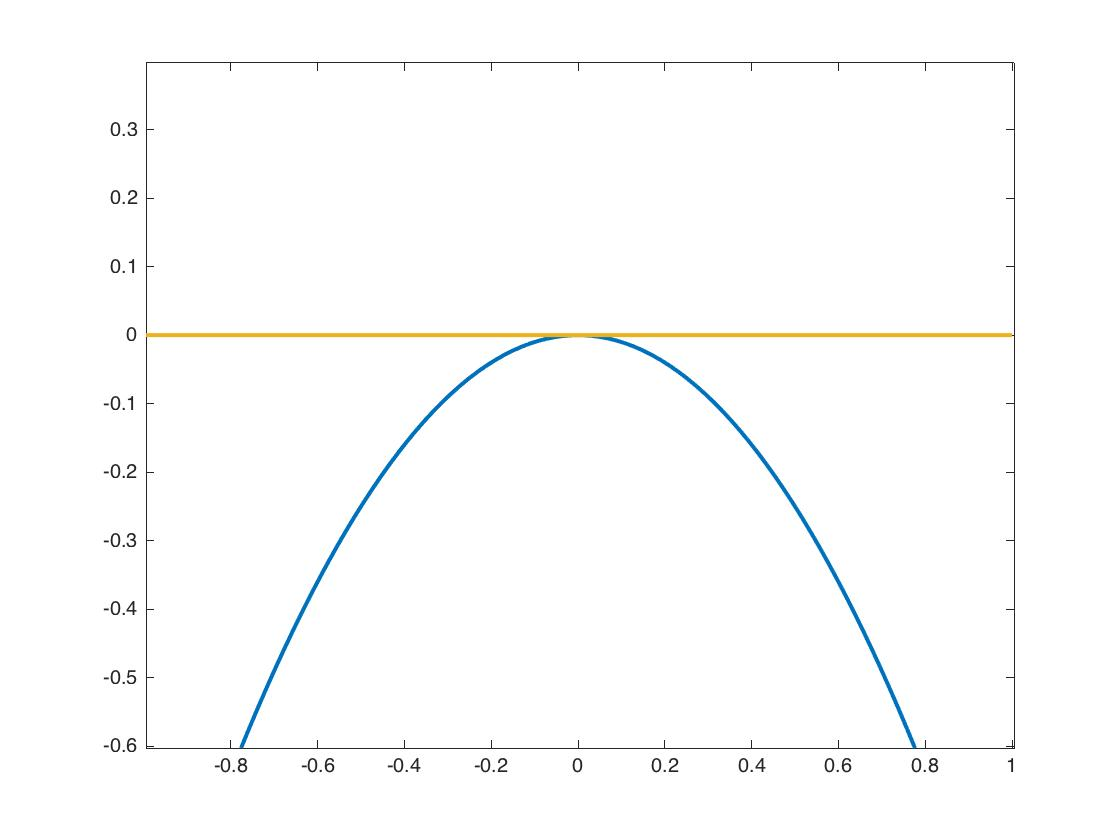
\includegraphics[width=0.7\textwidth]{subgrad1.jpg}
    \end{center}
    \begin{center}
        $f(x)=-x^2,\partial f(0)=\{0\}$.
    \end{center}
\end{frame}

\begin{frame}
    \frametitle{Example 2}
    \begin{center}
        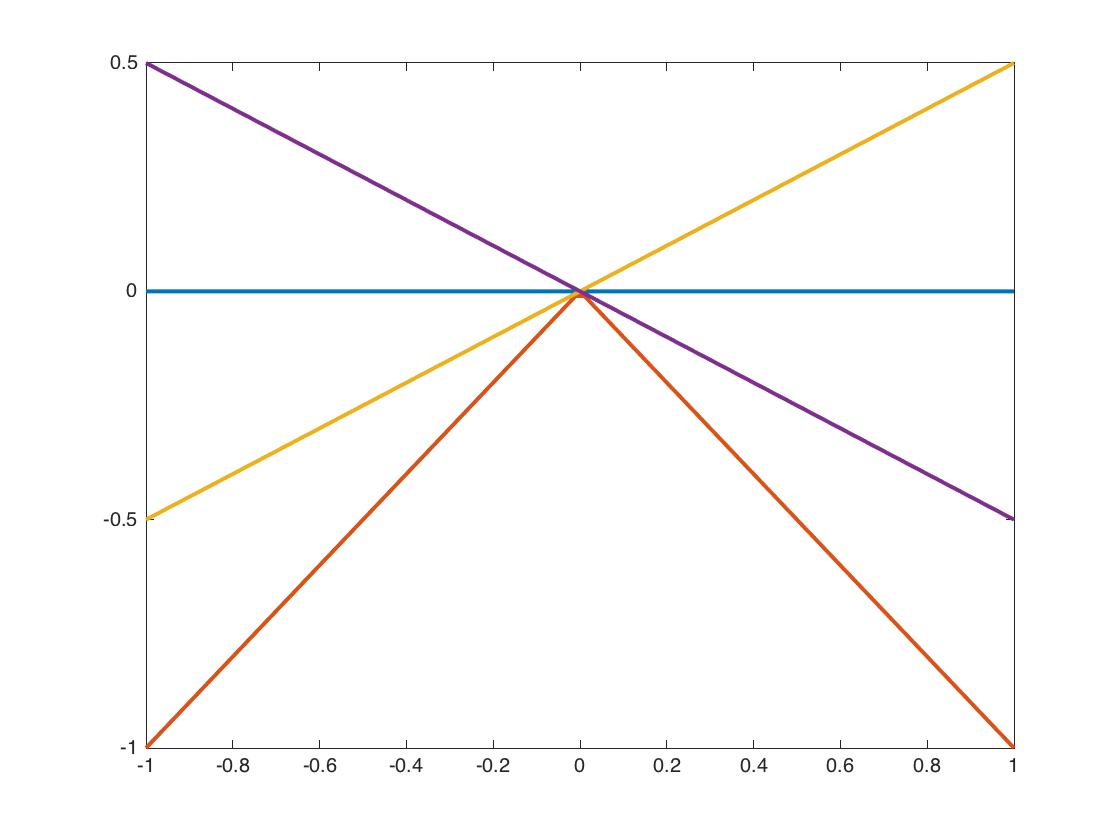
\includegraphics[width=0.7\textwidth]{subgrad2.jpg}
    \end{center}
    \begin{center}
        $f(x)=-|x|,\partial f(0)=[-1,1]$.
    \end{center}
\end{frame}

\begin{frame}
    \frametitle{Existence and Property of Subgradients}
    Suppose $f$ is concave. Then $\partial f(x)$ is non-empty for any $x\in \mathbf{int}\,\mathbf{dom}f$.

    \begin{equation}
        \begin{array}{cl}
             & x\in\arg\max f(x) \\
            \iff & \forall x'\in \mathbf{dom}\,f,f(x')\le f(x) \\
            \iff & \forall x'\in \mathbf{dom}\,f,f(x')\le f(x)+\langle0,x'-x\rangle \\
            \iff & 0\in\partial f(x).
        \end{array}
    \end{equation}
\end{frame}

\begin{frame}
\frametitle{Maximum of Convex Functions}
Suppose $\forall y\in \mathcal{A}$, $f(x,y)$ is convex in $x$. Then $g(x)=\sup_{y\in \mathcal{A}}f(x,y)$ is convex in $x$.
\begin{center}
    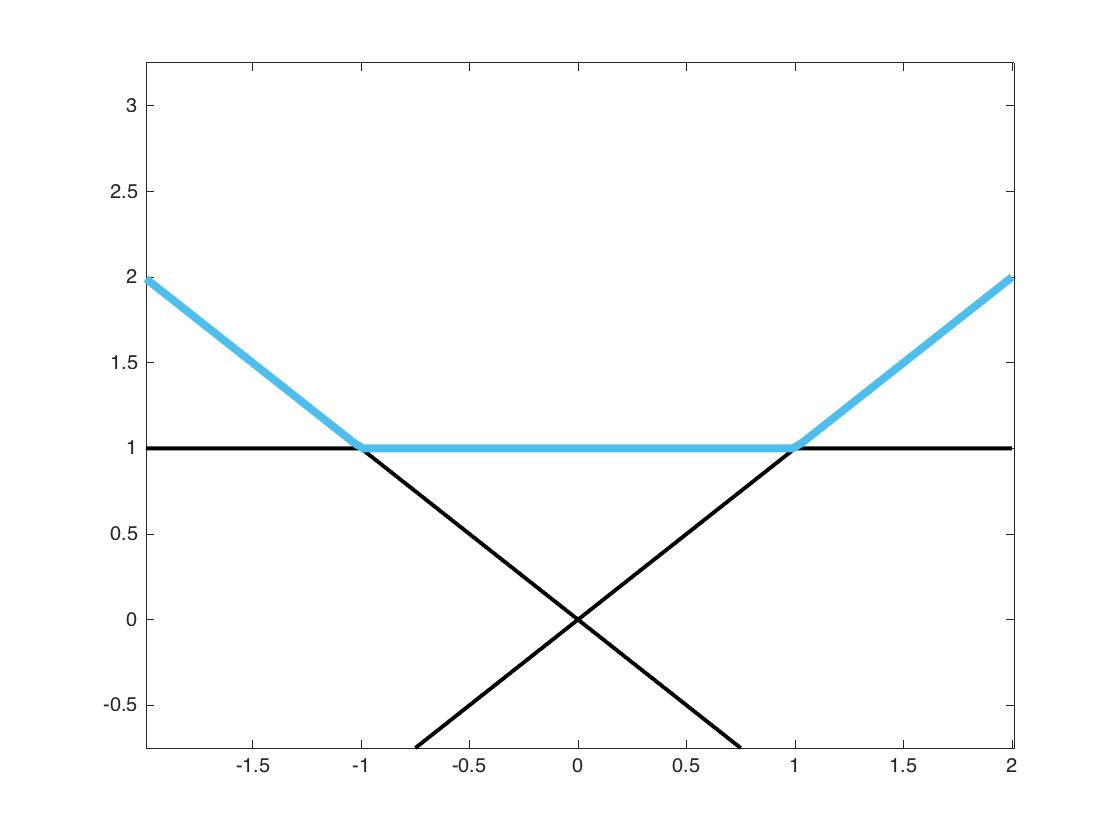
\includegraphics[width=0.7\textwidth]{convexmax.jpg}
\end{center}
\end{frame}

\begin{frame}
    \frametitle{Return to Social Welfare Maximizatoin}
    Recall that given price $p\in \mathbb{R}_+^m$,
    \begin{equation}
        x(p)=\arg\max_{x\in \mathcal{C}}u(x,p)=\arg\max_{x\in \mathcal{C}}(v(x)-\langle x,p\rangle).
    \end{equation}
    Let
    \begin{equation}
        s(p)=\max_{x\in \mathcal{C}}(v(x)-\langle x,p\rangle)=v(x(p))-\langle x(p),p\rangle.
    \end{equation}
    Note that $s(p)$ is a supreme of linear functions, thus $s(p)$ is \textbf{convex} in $p$.

    Actually $s(p)$ is closely related to the notion of \textbf{convex conjugate}. Although there is some difference, they share similar properties.
\end{frame}

\begin{frame}
    \frametitle{Relationship between conjugate functions}

    For every pair $(x,p)\in \mathcal{C}\times\mathbb{R}_+^m$ and $v$ which is concave and monotonically increasing,
    \begin{equation}
        \begin{array}{cl}
             & p \in \partial v(x)\iff x \in \arg\max_{x'\in \mathcal{C}} ( v(x')-\langle x',p\rangle ) \\
            \iff & -x \in \partial s(p)\iff p \in \arg\min_{p'\in \mathbb{R}_+^m} ( \langle x,p'\rangle + s(p') ).
        \end{array}
    \end{equation}
\end{frame}

\begin{frame}
    \frametitle{Proof}
    \begin{itemize}
        \item \begin{equation}
            \begin{array}{cl}
                 & x \in \arg\max_{x'\in \mathcal{C}} ( v(x')-\langle x',p\rangle ) \\
                \iff & 0\in\{y-p|y\in\partial v(x)\} \\
                \iff & p\in\partial v(x).
            \end{array}
        \end{equation}
        \item Similarly, $-x \in \partial s(p)\iff p \in \arg\min_{p'\in \mathbb{R}_+^m} ( \langle x,p'\rangle + s(p') )$.
    \end{itemize}
\end{frame}

\begin{frame}
    \frametitle{Proof}
    \begin{itemize}
        \item We now consider the relationship between $x \in \arg\max_{x'\in \mathcal{C}} ( v(x')-\langle x',p\rangle )$ and $p \in \arg\min_{p'\in \mathbb{R}_+^m} ( \langle x,p'\rangle + s(p') )$.

        Define
        \begin{equation}
            \begin{array}{rcl}
                L(x',p') & = & \langle x,p'\rangle+v(x')-\langle x',p'\rangle \\
                g(p') & = & \max_{x'\in \mathcal{C}}L(x',p').
            \end{array}
        \end{equation}

        By Sion's theorem,
        \begin{equation}
            \min_{p'\in \mathbb{R}_+^m}\max_{x'\in \mathcal{C}}L(x',p')=\max_{x'\in \mathcal{C}}\min_{p'\in \mathbb{R}_+^m}L(x',p').
        \end{equation}
    \end{itemize}
\end{frame}

\begin{frame}
    \begin{equation}
        \begin{array}{rcl}
            L(x',p') & = & \langle x,p'\rangle+v(x')-\langle x',p'\rangle \\
            g(p') & = & \max_{x'\in \mathcal{C}}L(x',p') \\
            \displaystyle\min_{p'\in \mathbb{R}_+^m}\max_{x'\in \mathcal{C}}L(x',p') &= & \displaystyle\max_{x'\in \mathcal{C}}\min_{p'\in \mathbb{R}_+^m}L(x',p').
        \end{array}
    \end{equation}
    RHS: $\max_{x'\in \mathcal{C}}v(x')$ subject to $x'\le x$, which is just $v(x)$ since $v$ is monotonically increasing.

    LHS:
    \begin{equation}
        \begin{array}{cl}
             & p\in\arg\min_{p'\in \mathbb{R}_+^m}g(p') \\
            \iff & g(p)=v(x)=L(x,p) \\
            \iff & x \in \arg\max_{x'\in \mathcal{C}} ( v(x')-\langle x',p\rangle ).
        \end{array}
    \end{equation}
\end{frame}

\begin{frame}
    \frametitle{Social Welfare Maximization}
    Recall we try to maximize $\mathrm{SW}(p)=v(x(p))-c(x(p))$ over $p\in\mathbb{R}_+^m$. But this may be a non-convex function in general.

    Actually we want to maximize $\mathrm{SW}(x)=v(x)-c(x)$ for those $x$ which can be induced by some price $p$. For $x\in \mathbb{R}_{++}^m,p\in\partial v(x)\iff x\in\arg\max_{x'\in \mathcal{C}} u(x',p)$.

    There are many ways to deal with the boundary; for simplicity, assume for any $x\in \mathcal{C}$, $\partial v(x)$ is nonempty, and thus we can just maximize $v(x)-c(x)$ over $\mathcal{C}$.
\end{frame}

\section{Algorithm}
\subsection{Subgradient Descent}

\begin{frame}
    \frametitle{Subgradient Descent}
    To maximize $f(x)$ over a convex compact set $\mathcal{C}$,
    \begin{enumerate}
        \item Pick $x_1$ from $\mathcal{C}$.
        \item for $t$ = $1$ to $T$:
        \begin{enumerate}
            \item Choose $g_t\in\partial f(xt)$.
            \item Let $x_{t+1}=\Pi_{\mathcal{C}}(x_t+\eta_tg_t)$.
        \end{enumerate}
    \end{enumerate}
\end{frame}

\begin{frame}
    \frametitle{Error Bound}
    Suppose the diameter of $\mathcal{C}$ is upper-bounded by $R$ and $f(x)$ is $\lambda$-Lipschitz over $\mathcal{C}$, then set $\eta_t=\frac{R}{\lambda\sqrt{T}}$ gives
    \begin{equation}
        f(\frac{1}{T}\sum_{t=1}^Tx_t)\ge\min_{x\in \mathcal{C}}f(x)-\frac{R\lambda}{\sqrt{T}}.
    \end{equation}
    In other words, to approximate the optimum of $f$ with an $\epsilon$ error, $(\frac{R\lambda}{\epsilon})^2$ steps suffice.

    We can do better with gradients, but more assumptions will be needed. For example, if $f$ is $\beta$-strongly smooth and concave, we need $O(\frac{1}{\epsilon})$ steps to get an $\epsilon$ error.
\end{frame}

\subsection{A Two-Level Subgradient Descent}
\begin{frame}
    \frametitle{Optimizing Using Dual Subgradients}
    \begin{itemize}
        \item We want to maximize $v(x)-c(x)$ over $\mathcal{C}$.

        \item Assume the subgradient of $c(x)$ can be computed efficiently. The seller can set price $p$, and observe $x(p)$. Recall that since $x(p)$ maximizes $u(x,p)$, $-x(p)\in\partial s(p)$.

        We don't known $v$, $\partial v$, $s$, but can compute $x(p)\in\partial s(p)$.

        \item However, for a fixed $x$, $p \in \partial v(x)\iff p \in \arg\min_{p'\in \mathbb{R}_+^m} ( \langle x,p'\rangle + s(p') )$.
\end{itemize}
\end{frame}

\begin{frame}
    \frametitle{A Two-Level Subgradient Descent}
    \begin{enumerate}
        \item Maximize $v(x)-c(x)$ using subgradient descent.
        \item For each $x^{(t)}$ in the above subgradient descent, compute $p\in\partial v(x)$ by minimizing $\langle x^{(t)},p'\rangle+s(p')$ using another subgradient descent.
    \end{enumerate}
\end{frame}

\begin{frame}
    \frametitle{More Technical Details}
    \begin{itemize}
        \item Given $x$, at the end of the lower-level subgradient we get some $\tilde{p}$ such that $g(\tilde{p})-g^*\le\epsilon$. Let $\tilde{x}=x(\tilde{p})$. Then $\tilde{p}\in\partial v(\tilde{x})$, but in general $\tilde{x}\ne x$! But $x\approx\tilde{x}$ is OK.

        A concave function $f$ is $\alpha$-strongly concave if $\forall x,y\in \mathbf{dom}\,f,\forall g\in\partial f(x), f(y)-f(x)\le \langle g,y-x\rangle-\frac{\alpha}{2}\|y-x\|_2^2$.

        If $x$ maximizes $f$, then $\frac{\alpha}{2}\|y-x\|_2^2\le f(x)-f(y)$.

        With the strong concavity assumption, we can get $x\approx\tilde{x}$ from $g^*\approx g(\tilde{p})$.
        \item $p$ needs to be bounded; this can be achieved by some continuity assumptions.
    \end{itemize}
\end{frame}

\section{Extensions}
\begin{frame}
    \frametitle{Extensions}
    \begin{itemize}
        \item Profit maximization: Assume $v$ is differentiable and homogeneous with degree $k$, which means that for any $x\in \mathbb{R}_+^m$ and $\sigma>0$, $v(\sigma x)=\sigma^k v(x)$. Then for $x\in \mathbf{int}\,\mathcal{C}$, only $\nabla v(x)$ will induce $x$, and $\langle\nabla v(x),x\rangle=kv(x)$.

        \item Distribution case: At each time step, a valuation is sampled from an unknown distribution. The peobability of $v_i$ is $q_i$. Then we can replace $v(x)$ in the previous discussion with $\sum_{i=1}^{n}q_iv_i(x_i)$ subject to $\sum_{i=1}^{n}q_ix_i\le x$.
    \end{itemize}
\end{frame}

\section{Open Directions}
\begin{frame}
    \frametitle{Open Directions}
    \begin{itemize}
        \item Budget contraint
        \item Non-quasi-linear utility
        \item Limited supply
        \item ...
    \end{itemize}
\end{frame}

\begin{frame}
\frametitle{References}
\footnotesize{
\begin{thebibliography}{99} % Beamer does not support BibTeX so references must be inserted manually as below
\bibitem[Smith, 2012]{p1} Roth A, Ullman J, Wu Z S.
\newblock Watch and learn: Optimizing from revealed preferences feedback
\newblock \emph{ACM SIGecom Exchanges} 14(1): 101-104.

\bibitem[Smith, 2012]{p1} Roth A, Slivkins A, Ullman J, et al.
\newblock Multidimensional Dynamic Pricing for Welfare Maximization
\newblock \emph{arXiv preprint} arXiv:1607.05397, 2016.
\end{thebibliography}
}
\end{frame}

%------------------------------------------------

\begin{frame}
\Huge{\centerline{The End}}
\end{frame}

%----------------------------------------------------------------------------------------

\end{document}
